%\vspace{-2in}

\begin{figure}[H]
\centering
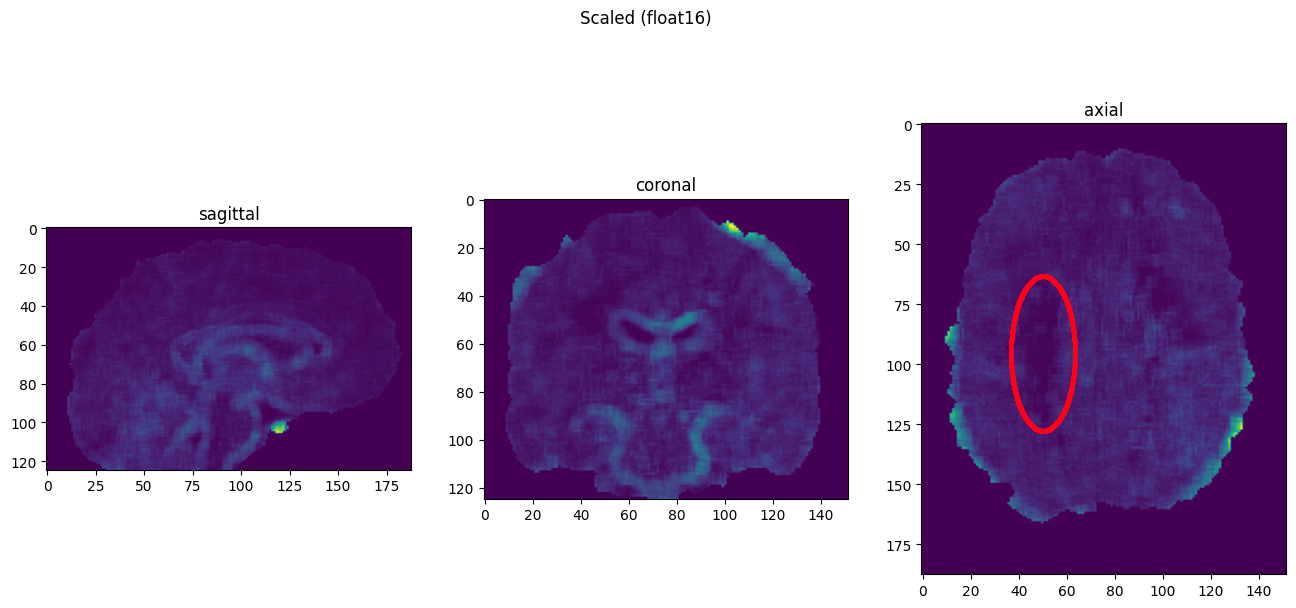
\includegraphics[width=0.9\textwidth]{rad_gldm_small_scale_16}
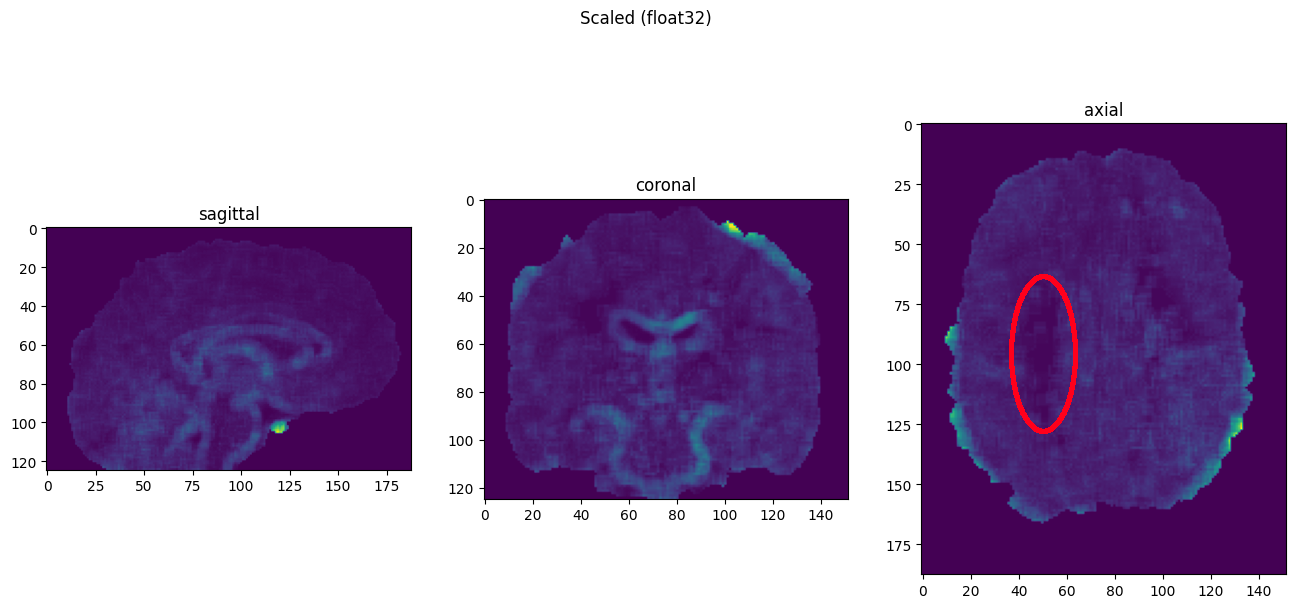
\includegraphics[width=0.9\textwidth]{rad_gldm_small_scale_32}
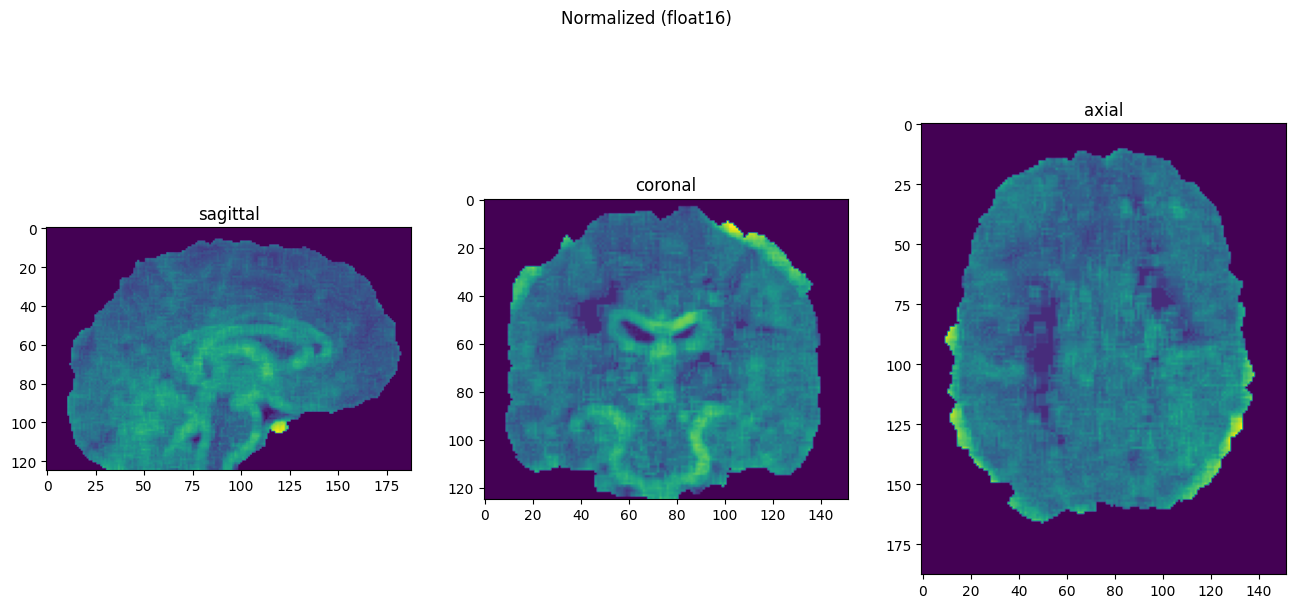
\includegraphics[width=0.9\textwidth]{rad_gldm_small_norm_16}
\caption{Slice: GLDM Small Dependence High Gray Level Emphasis}
\label{fig:gls}
\end{figure}

\begin{figure}[H]
\centering
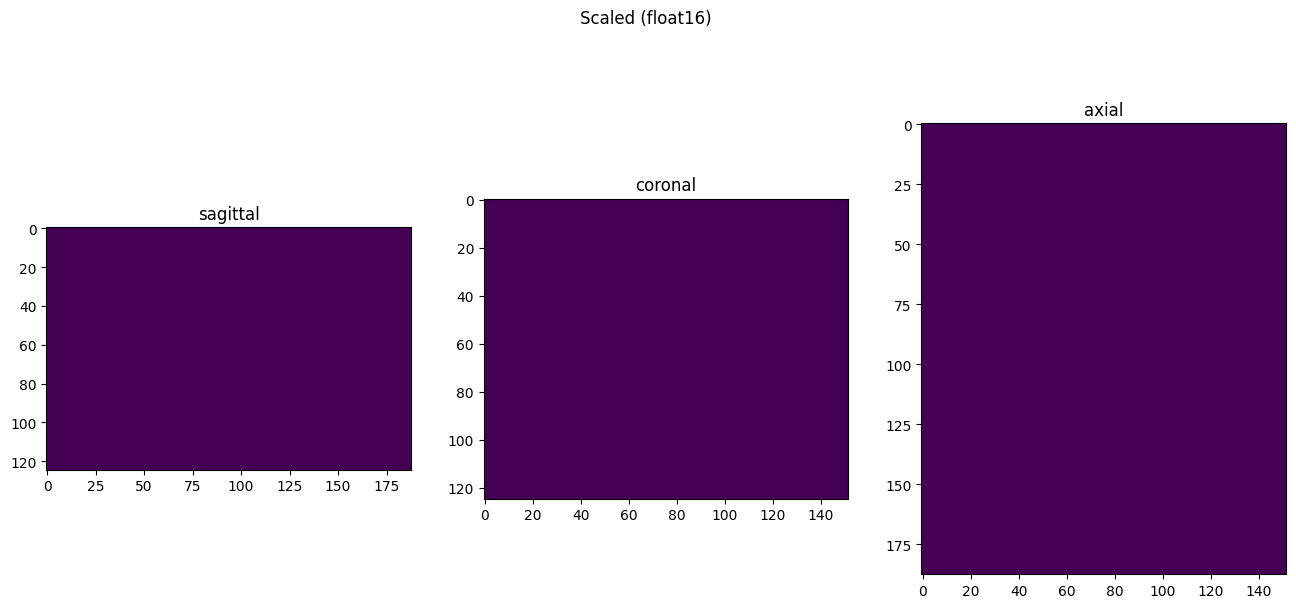
\includegraphics[width=0.9\textwidth]{rad_ngtdm_busyness_scale_16}
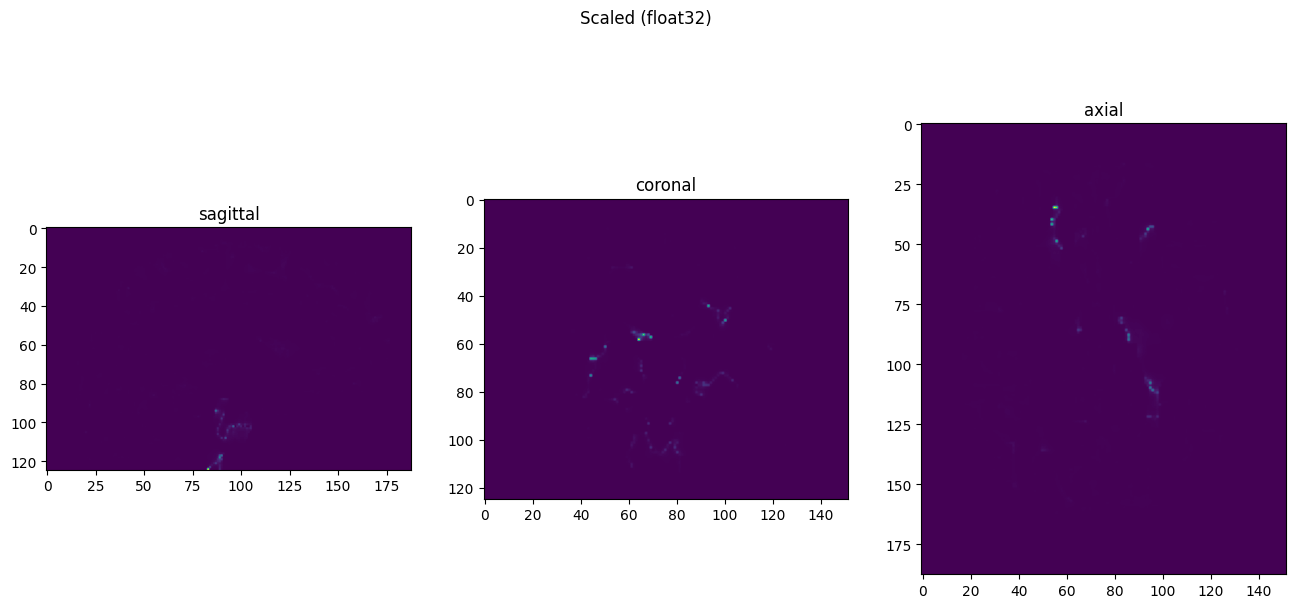
\includegraphics[width=0.9\textwidth]{rad_ngtdm_busyness_scale_32}
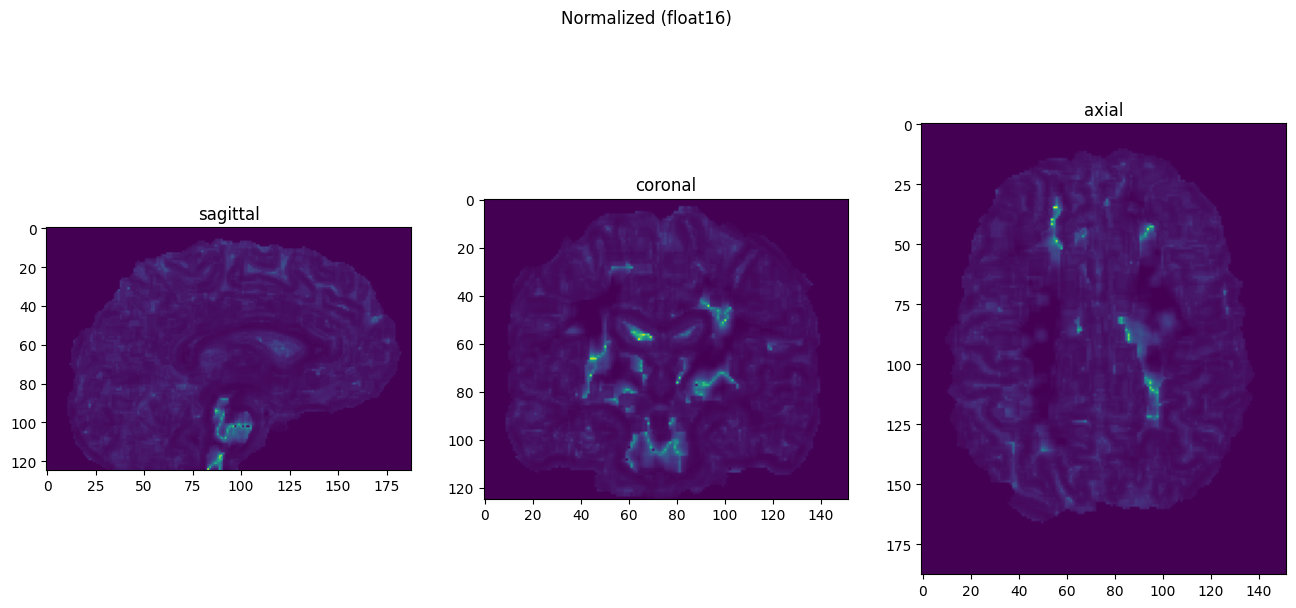
\includegraphics[width=0.9\textwidth]{rad_ngtdm_busyness_norm_16}
\caption{Slice: NGTDM Busyness}
\label{fig:ngb}
\end{figure}

\begin{figure}[H]
\centering
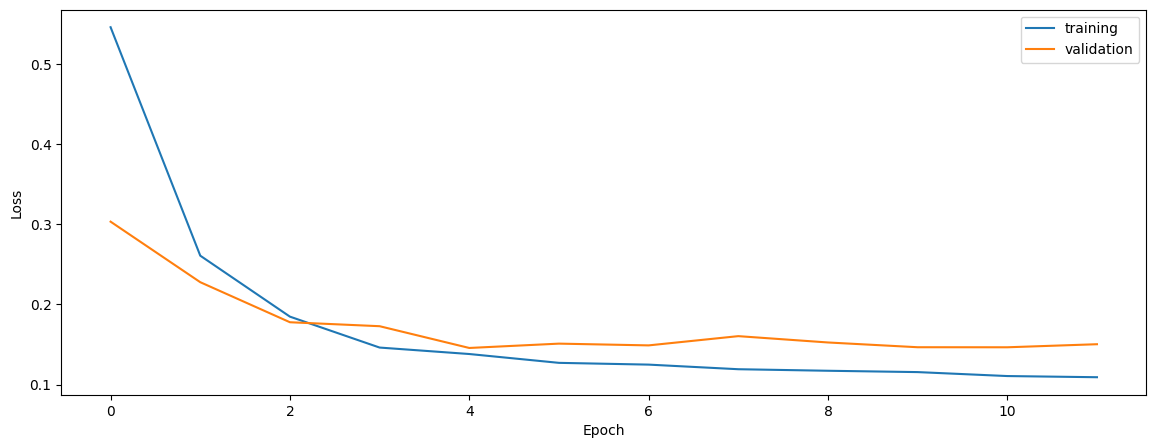
\includegraphics[width=0.7\textwidth]{subcortical_curve}
\caption{Training Curve: Subcortical}
\label{fig:curve-sub}
\end{figure}

\begin{figure}[H]
\centering
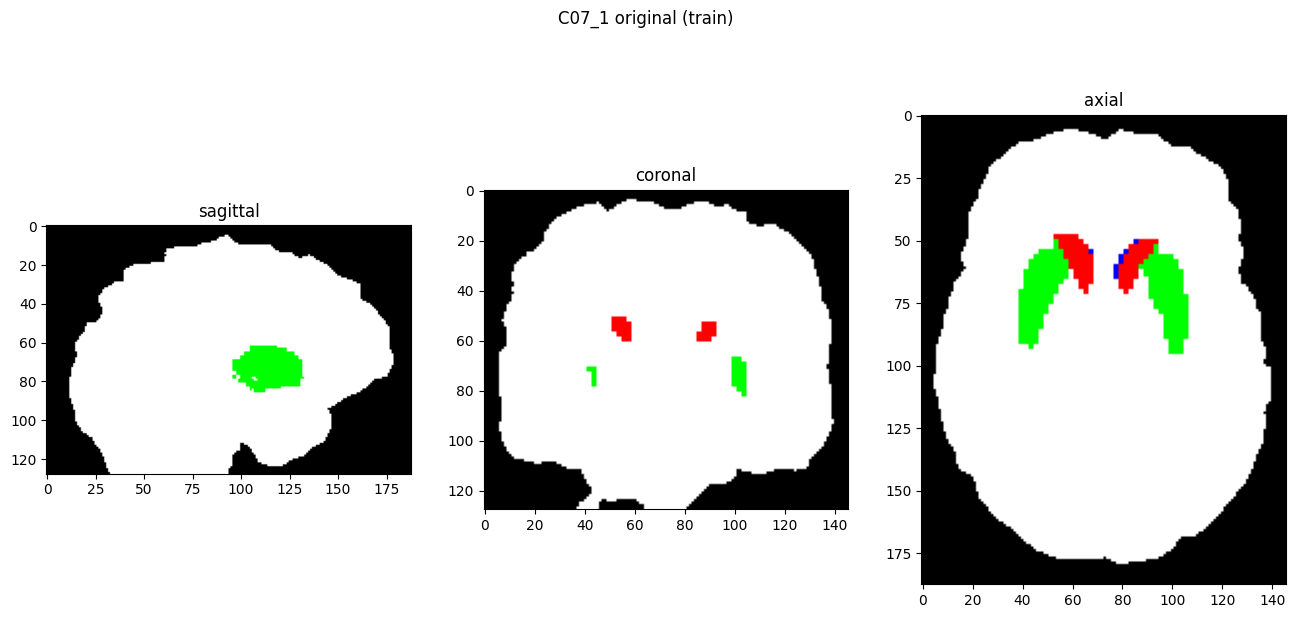
\includegraphics[width=0.9\textwidth]{subcortical_train_o}
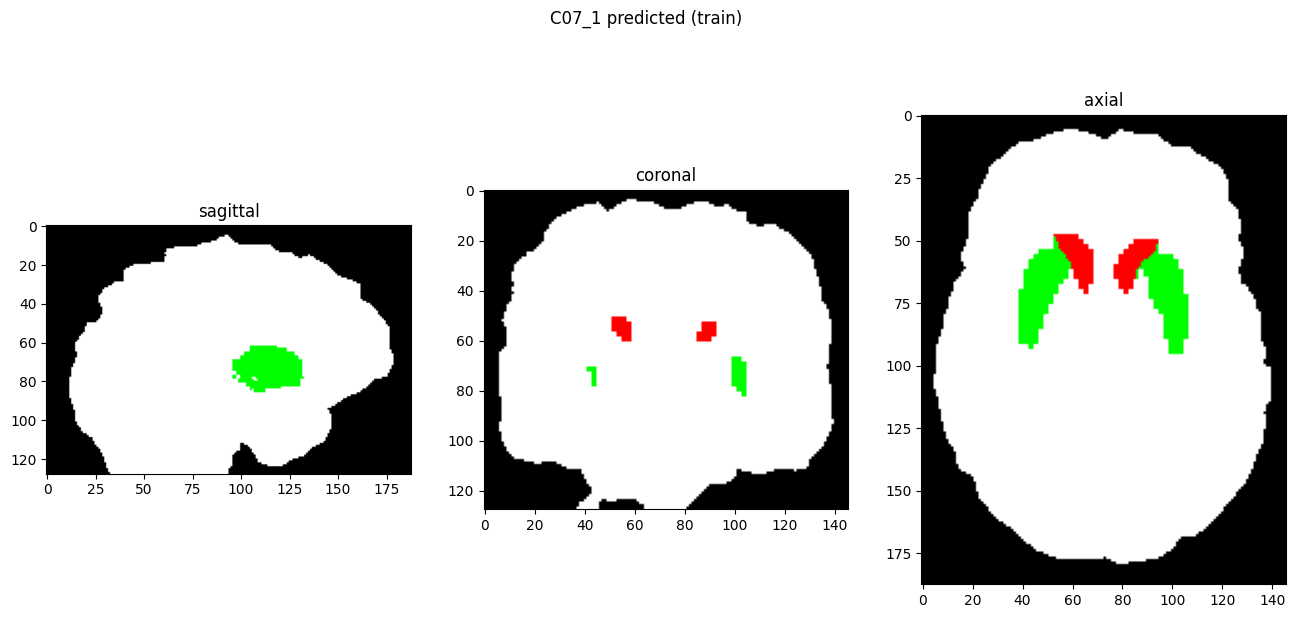
\includegraphics[width=0.9\textwidth]{subcortical_train_p}
\caption{Train Predictions: Subcortical}
\label{fig:pred-tra-sub}
\end{figure}

\begin{figure}[H]
\centering
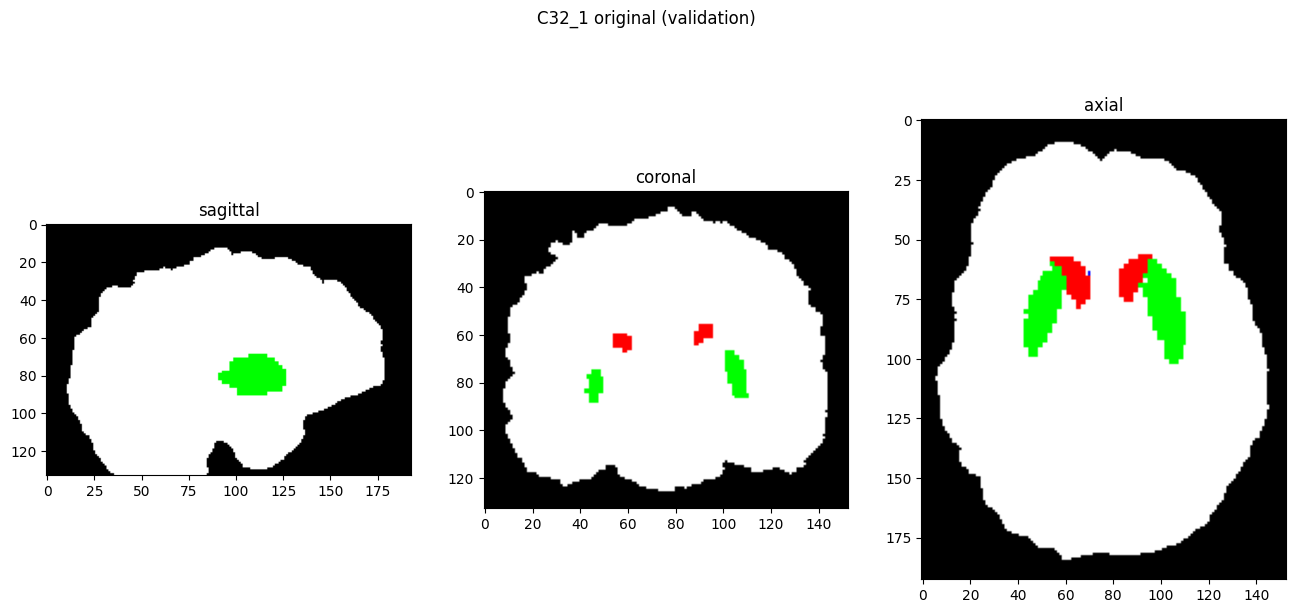
\includegraphics[width=0.9\textwidth]{subcortical_val_o}
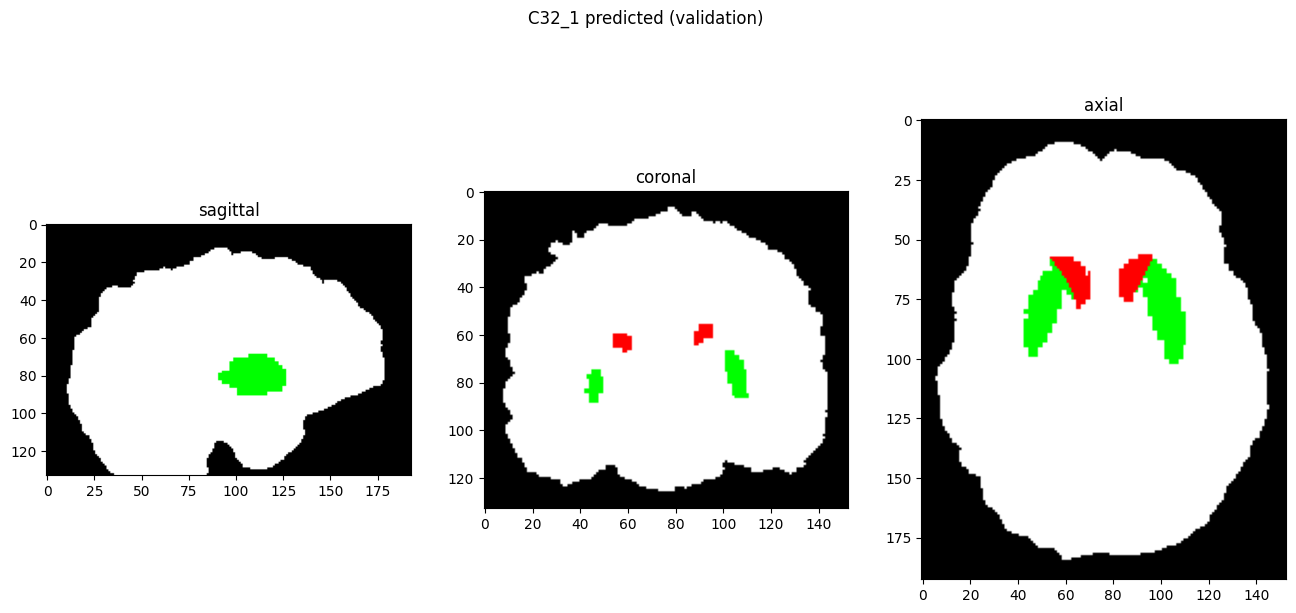
\includegraphics[width=0.9\textwidth]{subcortical_val_p}
\caption{Validation Predictions: Subcortical}
\label{fig:pred-val-sub}
\end{figure}

\begin{figure}[H]
\centering
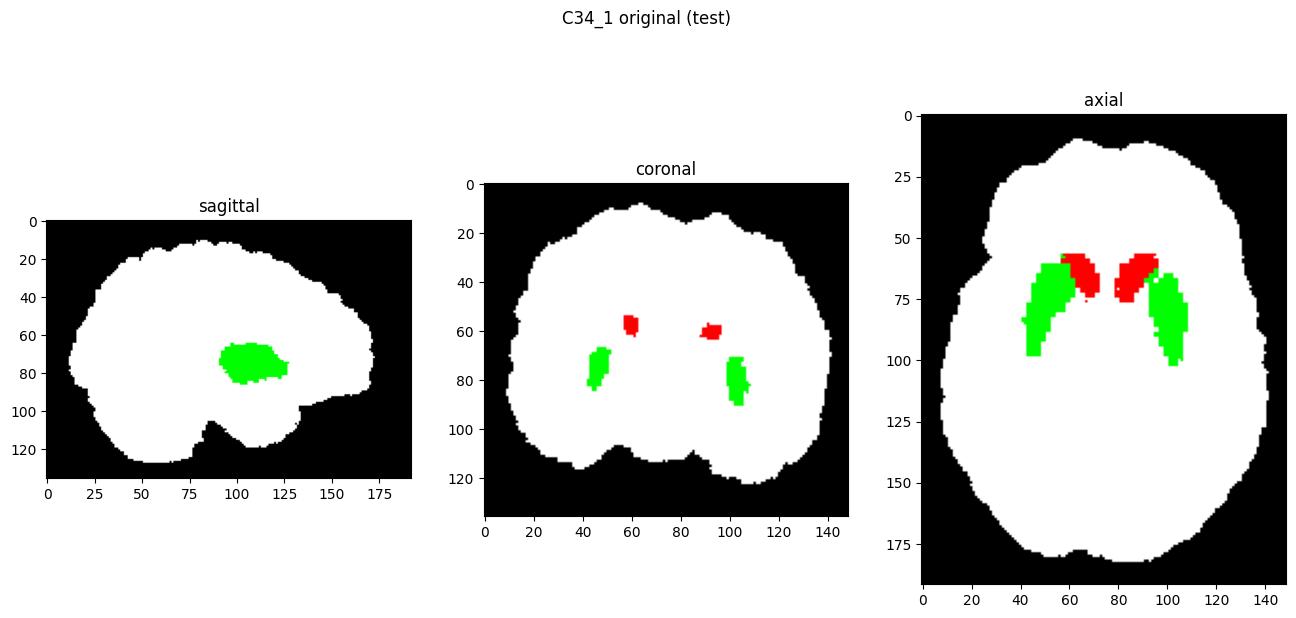
\includegraphics[width=0.9\textwidth]{subcortical_test_o}
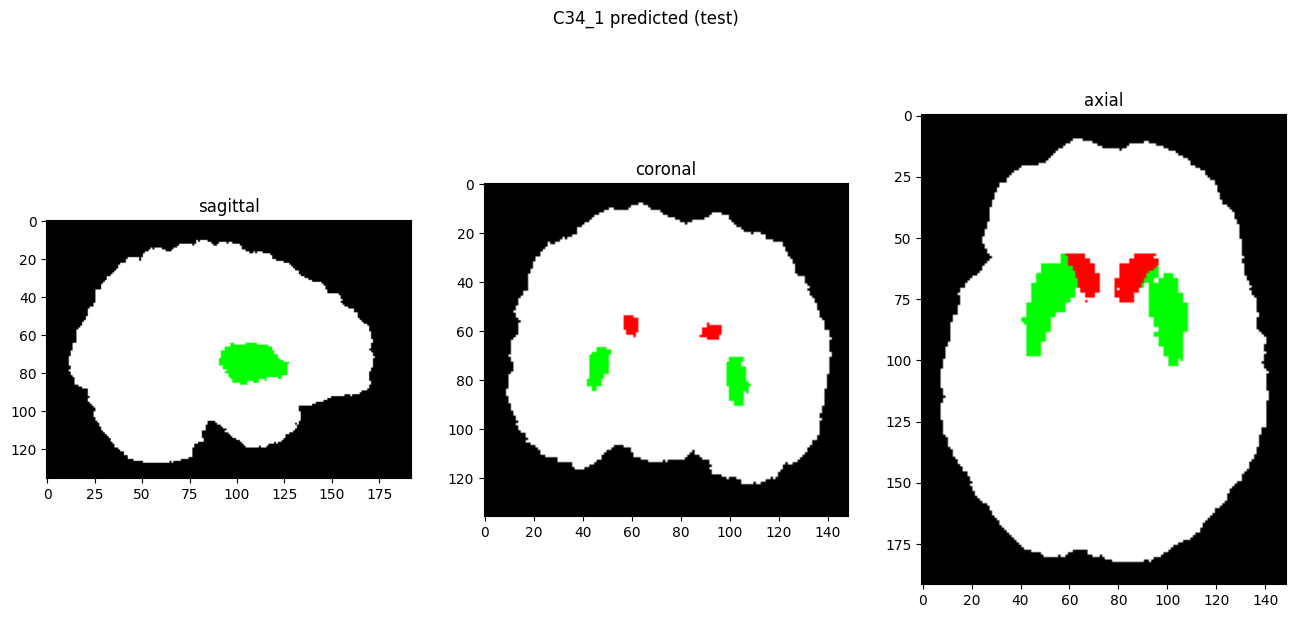
\includegraphics[width=0.9\textwidth]{subcortical_test_p}
\caption{Test Predictions: Subcortical}
\label{fig:pred-tes-sub}
\end{figure}




